\documentclass[11pt]{article}

\usepackage[a4paper,margin=1in]{geometry}
\usepackage{amsmath,amssymb,bm}
\usepackage{booktabs}
\usepackage{siunitx}
\usepackage{algorithm}
\usepackage{algpseudocode}
\usepackage{tikz}
\usetikzlibrary{arrows.meta,positioning,fit,backgrounds}
\usepackage[hidelinks]{hyperref}
\usepackage{xcolor}

\newcommand{\R}{\mathbf{R}}
\newcommand{\I}{\mathbf{I}}
\newcommand{\bp}{\mathbf{p}}
\newcommand{\bv}{\mathbf{v}}
\newcommand{\ba}{\mathbf{a}}
\newcommand{\bg}{\mathbf{g}}
\newcommand{\bomega}{\bm{\omega}}
\newcommand{\bq}{\mathbf{q}}
\newcommand{\bK}{\mathbf{K}}
\newcommand{\bH}{\mathbf{H}}
\newcommand{\bF}{\mathbf{F}}
\newcommand{\bP}{\mathbf{P}}
\newcommand{\bQ}{\mathbf{Q}}
\newcommand{\bz}{\mathbf{z}}
\newcommand{\bx}{\mathbf{x}}
\newcommand{\skewm}[1]{\lfloor #1 \rfloor_\times}
\newcommand{\dtheta}{\delta\bm{\theta}}
\newcommand{\dx}{\delta\bx}

\title{\textbf{A Consistency-Gated Quaternion Error-State Kalman Filter\\ for Multi-Sensor Inertial Navigation}}
\author{Irfan Saric}
\date{December 2025}

\begin{document}
\maketitle

\begin{abstract}
We describe the design, implementation, and verification of an error-state Kalman filter (ESKF)
that fuses a strapdown inertial measurement unit (IMU) with up to nine aiding modalities---GPS
position and Doppler velocity, a barometric altimeter, a magnetometer, a downward laser altimeter
(LiDAR), ultra-wideband (UWB) radio ranging, optical flow, a Doppler velocity log (DVL), and a
direct attitude fix---to estimate the pose of an aerial vehicle. The filter follows the
multiplicative, local error-state formulation of Sol\`a~\cite{sola2017} and Trawny and
Roumeliotis~\cite{trawny2005}: a nominal state carries the full estimate and is integrated directly
from the IMU, while a minimal $15$-dimensional error state, reset to zero after every correction,
carries the covariance. Each of the ten measurement models is given with its exact error-state
Jacobian, and every Jacobian is validated against a finite difference. The central claim is not
merely that the filter tracks well but that its \emph{reported uncertainty is correct}: we verify
this with the normalized estimation error squared (NEES) consistency test of Bar-Shalom
et~al.~\cite{barshalom2001}, run as a Monte-Carlo gate over many simulated flights and shown to hold
throughout each flight, not only in the mean. On the full nine-sensor fusion the filter is
statistically consistent (position NEES $2.85$ against an expected $3.0$; full-state NEES $16.2$
against $15.0$) at \SI{0.05}{\metre} position RMSE, while remaining faithful to inertial-navigation
error theory: with all aiding removed the position error grows without bound, and it is recovered to
sub-metre accuracy by any single position-fixing modality, including GPS-denied UWB ranging. A
recorded reference dataset and a replay tool accompany the filter, and the complete system---core,
simulator, and a real-time 3D visualization---runs in the browser via WebAssembly and WebGL2.
\end{abstract}

\section{Introduction}

Aided inertial navigation estimates a vehicle's position, velocity, and orientation by integrating
high-rate inertial measurements and correcting the accumulated drift with lower-rate aiding sensors
\cite{farrell2008,groves2013,titterton2004}. Orientation makes the problem subtle: a unit quaternion
has four components but only three degrees of freedom, so a filter that estimates it directly must
either enforce the unit-norm constraint or carry a covariance for a quantity that is not free to
move in four directions. The \emph{error-state} (or indirect, or multiplicative) Kalman filter
resolves this by estimating a minimal three-parameter rotation error in the tangent space of the
current attitude estimate~\cite{markley2003,sola2017}. This paper documents such a filter, its ten
measurement models, and---most importantly---the statistical test that proves its covariance honest.

The contribution is one of rigor and reproducibility rather than novelty of formulation. The filter
is a faithful implementation of the standard local-error ESKF, but (i) each of the ten measurement
Jacobians is finite-difference-checked; (ii) the whole estimation loop is gated on NEES consistency,
verified both in aggregate and as a function of time; (iii) a recorded reference dataset and a
replay harness make the results independently reproducible; and (iv) the entire system, from the
dependency-free numerical core to a real-time three-dimensional visualization, runs in the browser.
Source, the dataset, and an interactive demonstration are available at
\url{https://github.com/Zarathos94/ekf-sim} and \url{https://irfansaric.com/showcase/ekf-sim}.

\section{Related Work and Datasets}

The indirect Kalman filter for attitude dates to spacecraft navigation and is surveyed by
Markley~\cite{markley2003} and, in quaternion form, by Trawny and Roumeliotis~\cite{trawny2005} and
Sol\`a~\cite{sola2017}; it is the attitude workhorse of aided-INS texts~\cite{farrell2008,groves2013}.
For visual-inertial estimation the multi-state constraint Kalman filter (MSCKF) of Mourikis and
Roumeliotis~\cite{mourikis2007} keeps a sliding window of poses, and optimization-based systems such
as VINS-Mono~\cite{qin2018} and the factor-graph / incremental-smoothing approach of iSAM2 and
GTSAM~\cite{kaess2012,forster2017} trade recursion for re-linearization. The invariant EKF of Barrau
and Bonnabel~\cite{barrau2017} improves consistency by exploiting the group structure of the state;
the filter here uses the more common local-error parameterization but demonstrates consistency
empirically. Radio ranging with UWB for micro-aerial vehicles follows Mueller
et~al.~\cite{mueller2015}, and metric optical flow follows Honegger et~al.~\cite{honegger2013}.

Public datasets are the standard proving ground for such estimators: EuRoC MAV~\cite{burri2016} and
TUM-VI~\cite{schubert2018} provide synchronized IMU, stereo imagery, and millimetre-accurate motion
capture ground truth; UZH-FPV~\cite{delmerico2019} targets aggressive first-person-view flight; and
KITTI~\cite{geiger2013} provides automotive IMU, GNSS, and LiDAR. Because ground truth on such data
is itself an estimate and the sensor suites differ from ours, we validate against an \emph{analytic}
trajectory---where truth is exact---and additionally ship a recorded, replayable dataset
(Section~\ref{sec:sim}) so that our specific results are reproducible bit-for-bit.

\section{State Representation}

The \textbf{nominal state} collects position $\bp\in\mathbb{R}^3$, velocity $\bv\in\mathbb{R}^3$,
orientation as a Hamilton unit quaternion $\bq\in\mathbb{S}^3$ (body to world), and the
accelerometer and gyroscope biases $\ba_b,\bomega_b\in\mathbb{R}^3$:
\begin{equation}
  \bx = (\bp,\ \bv,\ \bq,\ \ba_b,\ \bomega_b).
\end{equation}
The \textbf{error state} is the $15$-vector
\begin{equation}
  \dx = (\delta\bp,\ \delta\bv,\ \dtheta,\ \delta\ba_b,\ \delta\bomega_b) \in \mathbb{R}^{15},
\end{equation}
where the rotation error $\dtheta$ is defined \emph{locally} (in the body frame) through the
multiplicative relation
\begin{equation}
  \bq_{\text{true}} = \bq \otimes \exp\!\left(\tfrac{1}{2}\dtheta\right),
  \label{eq:localerror}
\end{equation}
with $\exp(\cdot)$ the quaternion exponential map (Appendix~\ref{app:so3}) and $\otimes$ the
Hamilton product. The nominal state holds the full, unconstrained estimate; the error state, kept
near zero, holds a covariance $\bP\in\mathbb{R}^{15\times15}$ whose orientation block is an ordinary
$3\times3$ matrix. We write $\R=\R(\bq)$ for the rotation matrix and
$\skewm{\cdot}:\mathbb{R}^3\to\mathfrak{so}(3)$ for the skew-symmetric operator, so that
$\skewm{\ba}\bv = \ba\times\bv$.

Figure~\ref{fig:arch} shows the overall structure, and Algorithm~\ref{alg:eskf} the per-step loop.

\begin{figure}[h]
  \centering
  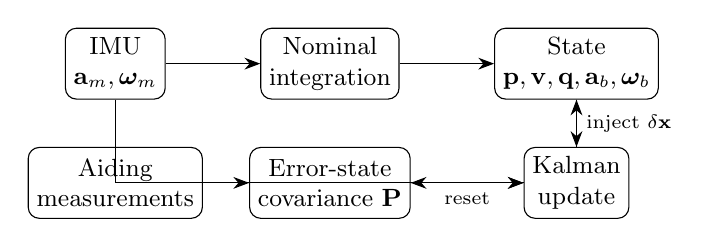
\begin{tikzpicture}[
    node distance=6mm and 12mm,
    box/.style={draw, rounded corners, align=center, minimum height=9mm, font=\small, inner sep=3pt},
    >={Stealth[length=2mm]}]
    \node[box] (imu) {IMU\\$\ba_m,\bomega_m$};
    \node[box, right=of imu] (nom) {Nominal\\integration};
    \node[box, right=of nom] (state) {State\\$\bp,\bv,\bq,\ba_b,\bomega_b$};
    \node[box, below=of nom] (cov) {Error-state\\covariance $\bP$};
    \node[box, below=of state] (upd) {Kalman\\update};
    \node[box, below=of imu] (meas) {Aiding\\measurements};
    \draw[->] (imu) -- (nom);
    \draw[->] (nom) -- (state);
    \draw[->] (imu) |- (cov) node[midway,above,font=\scriptsize] {};
    \draw[->] (cov) -- (upd);
    \draw[->] (meas) -- (upd);
    \draw[->] (state) -- (upd);
    \draw[->] (upd) -- node[right,font=\scriptsize] {inject $\delta\bx$} (state);
    \draw[->] (upd.west) -- node[below,font=\scriptsize] {reset} (cov.east);
  \end{tikzpicture}
  \caption{The error-state filter. The IMU drives the nominal state forward and inflates the
  error-state covariance; each aiding measurement produces a correction that is injected into the
  nominal state, after which the error state is reset to zero.}
  \label{fig:arch}
\end{figure}

\begin{algorithm}[h]
\caption{Error-state Kalman filter, one cycle}
\label{alg:eskf}
\begin{algorithmic}[1]
\State \textbf{Predict} (each IMU sample): integrate $\bp,\bv,\bq$; set $\bP \gets \bF\bP\bF^{\!\top}+\bQ$
\ForAll{available measurements $\bz$ with model $h$, Jacobian $\bH$, noise $\bm{R}$}
  \State $\bm{S} \gets \bH\bP\bH^{\!\top}+\bm{R}$;\quad $\bK \gets \bP\bH^{\!\top}\bm{S}^{-1}$;\quad $\dx \gets \bK(\bz-h(\bx))$
  \State \textbf{Inject}: $\bx \gets \bx \boxplus \dx$;\quad reset $\dx \gets 0$;\quad $\bP \gets \bm{G}\bP\bm{G}^{\!\top}$
  \State $\bP \gets (\I-\bK\bH)\bP(\I-\bK\bH)^{\!\top}+\bK\bm{R}\bK^{\!\top}$ \Comment{Joseph form}
\EndFor
\end{algorithmic}
\end{algorithm}

\section{Propagation}

At each IMU sample (rate $\approx\SI{200}{\hertz}$, interval $\Delta t$) with accelerometer reading
$\ba_m$ and gyroscope reading $\bomega_m$, define the bias-corrected specific force and body rate
$\ba = \ba_m - \ba_b$ and $\bomega = \bomega_m - \bomega_b$.

\paragraph{Nominal integration.} With gravity $\bg = (0,0,-\SI{9.80665}{\metre\per\second\squared})$,
\begin{align}
  \bp &\leftarrow \bp + \bv\,\Delta t + \tfrac{1}{2}(\R\ba + \bg)\,\Delta t^2, &
  \bv &\leftarrow \bv + (\R\ba + \bg)\,\Delta t, &
  \bq &\leftarrow \bq \otimes \exp\!\left(\tfrac{1}{2}\bomega\,\Delta t\right),
\end{align}
with the quaternion renormalized after each step.

\paragraph{Error-state transition.} $\dx \leftarrow \bF\,\dx$ with the block matrix
\begin{equation}
  \bF =
  \begin{bmatrix}
    \I & \I\,\Delta t & \mathbf{0} & \mathbf{0} & \mathbf{0} \\
    \mathbf{0} & \I & -\R\skewm{\ba}\,\Delta t & -\R\,\Delta t & \mathbf{0} \\
    \mathbf{0} & \mathbf{0} & \exp(-\skewm{\bomega}\,\Delta t) & \mathbf{0} & -\I\,\Delta t \\
    \mathbf{0} & \mathbf{0} & \mathbf{0} & \I & \mathbf{0} \\
    \mathbf{0} & \mathbf{0} & \mathbf{0} & \mathbf{0} & \I
  \end{bmatrix},
  \label{eq:F}
\end{equation}
in which the velocity--orientation coupling $-\R\skewm{\ba}$ is the first-order effect of an
orientation error on the rotated specific force, and the orientation block
$\exp(-\skewm{\bomega}\Delta t)$ is the exact rotation integral (Appendix~\ref{app:so3}) rather than
its first-order truncation~\cite{sola2017}.

\paragraph{Process noise.} $\bP \leftarrow \bF\bP\bF^{\!\top} + \bQ$ with
\begin{equation}
  \bQ = \operatorname{diag}\!\big(\mathbf{0},\ \sigma_a^2\Delta t^2\,\I,\ \sigma_g^2\Delta t^2\,\I,\
  \sigma_{ab}^2\Delta t\,\I,\ \sigma_{\omega b}^2\Delta t\,\I\big).
\end{equation}
The IMU white-noise terms scale as $\Delta t^2$: a per-sample noise of standard deviation $\sigma$
perturbs the integrated velocity or orientation by $\sigma\Delta t$ over the step, injecting a
variance $\sigma^2\Delta t^2$---also the only dimensionally consistent choice. The bias random walks
scale as $\Delta t$. A mis-scaled $\bQ$ is invisible in the RMSE but glaring in the NEES of
Section~\ref{sec:nees}.

\section{Measurement Updates}

For a measurement $\bz = h(\bx) + \bm{\nu}$, $\bm{\nu}\sim\mathcal{N}(0,\bm{R})$, the Jacobian
$\bH = \partial h / \partial \dx$ is evaluated at the nominal state and applied through
Algorithm~\ref{alg:eskf}. The ten models, with the non-zero blocks of $\bH$, are:

\begin{itemize}
  \item \textbf{GPS position}: $h = \bp$; $\ \partial h/\partial\delta\bp = \I_3$.
  \item \textbf{GPS Doppler velocity}: $h = \bv$; $\ \partial h/\partial\delta\bv = \I_3$.
  \item \textbf{Barometer} (altitude): $h = \bm{e}_3^{\top}\bp$; $\ \partial h/\partial\delta\bp = \bm{e}_3^{\top}$.
  \item \textbf{Magnetometer}: $h = \R^{\!\top}\bm{m}$ ($\bm{m}$ the world field);
        $\ \partial h/\partial\dtheta = \skewm{\R^{\!\top}\bm{m}}$, i.e.\ heading from the full vector.
  \item \textbf{LiDAR altimeter}: slant range to flat ground, $h = p_z / R_{33}$ with
        $R_{33} = \bm{e}_3^{\top}\R\,\bm{e}_3$; $\ \partial h/\partial p_z = 1/R_{33}$ and
        $\partial h/\partial\dtheta = -\frac{p_z}{R_{33}^2}[-R_{32},R_{31},0]$, so a single beam
        senses height \emph{and} tilt.
  \item \textbf{UWB radio ranging}: $h = \lVert\bp-\bm{b}_k\rVert$ to beacon $\bm{b}_k$;
        $\ \partial h/\partial\delta\bp = \hat{\bm{u}}^{\top}$, the unit line of sight. Position-only,
        so a few beacons localize with no GPS~\cite{mueller2015}.
  \item \textbf{Optical flow}: $h = \Pi\,\R^{\!\top}\bv$ ($\Pi$ the top two rows);
        $\ \partial h/\partial\delta\bv = \Pi\R^{\!\top}$, $\partial h/\partial\dtheta = \Pi\skewm{\R^{\!\top}\bv}$
        \cite{honegger2013}.
  \item \textbf{Doppler velocity (DVL)}: the full body-frame velocity $h = \R^{\!\top}\bv$;
        $\ \partial h/\partial\delta\bv = \R^{\!\top}$, $\partial h/\partial\dtheta = \skewm{\R^{\!\top}\bv}$.
  \item \textbf{Attitude fix} (star tracker / vision): a measured orientation $\bz_q$; the innovation
        is $\log(\bq^{-1}\!\otimes\bz_q)$ and $\partial h/\partial\dtheta = \I_3$---the standard
        multiplicative attitude update.
\end{itemize}

Every Jacobian is checked in the test suite against a central finite difference across all $15$
error directions, agreeing to $10^{-4}$; the attitude and velocity updates are additionally verified
to converge from a seeded error, which fails if a sign is wrong. All updates use the Joseph-form
covariance step of Algorithm~\ref{alg:eskf}, which stays symmetric positive-definite under finite
precision.

\section{Injection and Reset}
\label{sec:inject}

The correction is folded into the nominal state and the error reset to zero:
\begin{equation}
  \bp \leftarrow \bp + \delta\bp,\quad
  \bv \leftarrow \bv + \delta\bv,\quad
  \bq \leftarrow \bq\otimes\exp\!\left(\tfrac12\dtheta\right),\quad
  \ba_b \leftarrow \ba_b + \delta\ba_b,\quad
  \bomega_b \leftarrow \bomega_b + \delta\bomega_b .
\end{equation}
Because the linearization point of the orientation error moves onto the new nominal quaternion, the
covariance is transformed by the reset Jacobian
$\bm{G} = \operatorname{diag}(\I,\I,\ \I-\tfrac12\skewm{\dtheta},\ \I,\I)$,
$\ \bP \leftarrow \bm{G}\,\bP\,\bm{G}^{\!\top}$. Retaining the $\I-\tfrac12\skewm{\dtheta}$ term---often
dropped---is one of the details the consistency test rewards.

\section{Consistency: The NEES Gate}
\label{sec:nees}

The decisive test is \emph{statistical consistency}~\cite{barshalom2001}: the normalized estimation
error squared $\varepsilon = \bm{e}^{\top}\bP^{-1}\bm{e}$, where $\bm{e}$ is the estimation error
expressed in the filter's own $15$-dimensional tangent space (position and velocity differences, the
body-frame logarithmic map for orientation, and bias differences). For a consistent filter,
$\mathbb{E}[\varepsilon] = \dim$. Averaged over $N$ independent Monte-Carlo runs,
$N\bar\varepsilon \sim \chi^2(N\cdot\dim)$, giving the two-sided $95\%$ acceptance interval
\begin{equation}
  \bar\varepsilon \in
  \left[\ \frac{\chi^2_{0.025}(N\cdot\dim)}{N},\ \frac{\chi^2_{0.975}(N\cdot\dim)}{N}\ \right].
  \label{eq:neesband}
\end{equation}
Overconfidence lands above the band, conservatism below. The runs are seeded from a realistic
initial error drawn from the initial covariance, so the test scores the filter and not an omniscient
initialization; and the NEES is reported per five-second window as well as pooled, because
consistency must hold throughout the flight, not only in the mean.

\section{Simulation Environment and Test Data}
\label{sec:sim}

Ground truth is an analytic banking helical trajectory---a horizontal orbit of radius \SI{40}{\metre}
and period \SI{30}{\second} with a superimposed vertical oscillation---so position, velocity, and
acceleration are exact. Orientation follows a coordinated turn (nose along velocity, rolled into the
turn by the bank angle that balances lateral acceleration against gravity), and the body angular rate
is obtained by central-differencing the quaternion path. From this truth a strapdown IMU and the nine
aiding sensors are synthesized, each with configurable noise, bias walk, rate, and availability. A
\texttt{record} command writes the raw IMU stream, every aiding measurement, and ground truth to CSV;
a \texttt{replay} command re-runs the filter on that CSV and re-derives the RMSE and NEES, so the
dataset is an independently verifiable artifact rather than a live-only result.

\section{Results}

Table~\ref{tab:nees} reports the Monte-Carlo consistency check over $40$ flights of \SI{30}{\second}
with all nine sensors active; both the position and full-state NEES fall inside the band of
\eqref{eq:neesband}, and (not shown) each five-second window is independently within a
$[2.0,4.2]$ position-NEES band, so consistency holds throughout. The time-averaged RMSE is
\SI{0.049}{\metre} in position, \SI{0.021}{\metre\per\second} in velocity, and \SI{0.11}{\degree} in
attitude; replaying the recorded dataset reproduces \SI{0.046}{\metre}.

\begin{table}[h]
  \centering
  \begin{tabular}{lccc}
    \toprule
    Quantity & NEES mean & Expected & $95\%$ band \\
    \midrule
    Position (3-DOF)   & $2.85$  & $3.0$  & $[2.29,\ 3.81]$ \\
    Full state (15-DOF) & $16.23$ & $15.0$ & $[13.35,\ 16.74]$ \\
    \bottomrule
  \end{tabular}
  \caption{NEES consistency over $40$ Monte-Carlo flights, nine sensors active. Both statistics lie
  inside the band---the reported uncertainty is neither over- nor under-confident.}
  \label{tab:nees}
\end{table}

Table~\ref{tab:scenarios} shows steady-state RMSE as the sensor suite is changed. With \emph{all}
aiding removed the filter dead-reckons on the IMU alone and the position error reaches hundreds of
metres over \SI{30}{\second}---the quadratic error growth that accelerometer and gyroscope bias
predict for an unaided strapdown system~\cite{groves2013}. Any single position-fixing modality
restores sub-metre accuracy: GPS-denied UWB ranging recovers from \SI{16.6}{\metre} to
\SI{0.16}{\metre}, and the indoor and vision-aided suites---using no GPS at all---stay well under a
metre.

\begin{table}[h]
  \centering
  \begin{tabular}{lccc}
    \toprule
    Scenario & Position (m) & Velocity (m/s) & Attitude (\si{\degree}) \\
    \midrule
    Nominal (GPS + baro + mag)        & $0.47$   & $0.24$  & $0.99$ \\
    IMU only (dead reckoning)         & $\sim\!300$ & $25$ & $8.3$  \\
    GPS dropout                       & $16.6$   & $1.87$  & $2.05$ \\
    GPS denied $+$ UWB ranging        & $0.16$   & $0.10$  & $0.61$ \\
    Indoor (UWB $+$ LiDAR $+$ flow)   & $0.20$   & $0.10$  & $0.60$ \\
    Vision-aided (attitude $+$ DVL)   & $0.30$   & $0.09$  & $0.20$ \\
    Full fusion (all $9$ sensors)     & $0.05$   & $0.02$  & $0.11$ \\
    \bottomrule
  \end{tabular}
  \caption{Steady-state RMSE by scenario (mean of $12$ flights of \SI{30}{\second} each). Dead
  reckoning diverges; any single position fix, including UWB alone, recovers it.}
  \label{tab:scenarios}
\end{table}

\section{Conclusion}

We have presented a quaternion error-state Kalman filter fusing up to nine aiding sensors for
inertial navigation, in the standard local-error formulation, with each of the ten measurement
Jacobians derived and finite-difference-verified. The emphasis throughout is that correctness is
\emph{demonstrated}, not asserted: the full estimation loop passes a Monte-Carlo NEES consistency
gate in aggregate and over time, and the filter reproduces the expected inertial-navigation
behavior---unbounded dead-reckoning drift, and graceful recovery from any single position aid,
including GPS-denied ranging. A recorded dataset and a replay tool make the results reproducible, and
the complete system runs in the browser.

\appendix
\section{The SO(3) Exponential and the Discrete Transition}
\label{app:so3}

For a rotation vector $\bm{\phi}\in\mathbb{R}^3$ with $\theta=\lVert\bm{\phi}\rVert$ and
$\hat{\bm{\phi}}=\bm{\phi}/\theta$, the group exponential is Rodrigues' formula
\begin{equation}
  \exp(\skewm{\bm{\phi}}) = \I + \frac{\sin\theta}{\theta}\skewm{\bm{\phi}}
  + \frac{1-\cos\theta}{\theta^2}\skewm{\bm{\phi}}^2,
\end{equation}
with the small-angle limit $\I+\skewm{\bm{\phi}}$; the corresponding unit quaternion is
$\exp(\tfrac12\bm{\phi}) = \big(\cos\tfrac{\theta}{2},\ \sin\tfrac{\theta}{2}\,\hat{\bm{\phi}}\big)$.
The orientation block of \eqref{eq:F} is $\exp(-\skewm{\bomega}\Delta t)$ evaluated with this formula
rather than truncated, which matters at the high body rates of aggressive flight. The inverse (the
logarithmic map) recovers the rotation vector from a unit quaternion $(w,\bm{v})$ as
$2\,\mathrm{atan2}(\lVert\bm{v}\rVert, w)\,\bm{v}/\lVert\bm{v}\rVert$, and defines the box-minus used
to form the orientation component of the estimation error in Section~\ref{sec:nees}.

\begin{thebibliography}{99}

\bibitem{kalman1960}
R.~E. Kalman, ``A new approach to linear filtering and prediction problems,''
\emph{J. Basic Eng.}, vol.~82, no.~1, pp.~35--45, 1960.

\bibitem{sola2017}
J.~Sol\`a, ``Quaternion kinematics for the error-state Kalman filter,'' arXiv:1711.02508, 2017.

\bibitem{trawny2005}
N.~Trawny and S.~I. Roumeliotis, ``Indirect Kalman filter for 3D attitude estimation,''
Univ.\ of Minnesota, Tech.\ Rep.\ 2005-002, 2005.

\bibitem{markley2003}
F.~L. Markley, ``Attitude error representations for Kalman filtering,''
\emph{J. Guidance, Control, and Dynamics}, vol.~26, no.~2, pp.~311--317, 2003.

\bibitem{barshalom2001}
Y.~Bar-Shalom, X.~R. Li, and T.~Kirubarajan, \emph{Estimation with Applications to Tracking and
Navigation}. New York: Wiley, 2001.

\bibitem{farrell2008}
J.~A. Farrell, \emph{Aided Navigation: GPS with High Rate Sensors}. New York: McGraw-Hill, 2008.

\bibitem{groves2013}
P.~D. Groves, \emph{Principles of GNSS, Inertial, and Multisensor Integrated Navigation Systems},
2nd~ed. Boston: Artech House, 2013.

\bibitem{titterton2004}
D.~H. Titterton and J.~L. Weston, \emph{Strapdown Inertial Navigation Technology}, 2nd~ed. IET, 2004.

\bibitem{mourikis2007}
A.~I. Mourikis and S.~I. Roumeliotis, ``A multi-state constraint Kalman filter for vision-aided
inertial navigation,'' in \emph{IEEE ICRA}, 2007, pp.~3565--3572.

\bibitem{qin2018}
T.~Qin, P.~Li, and S.~Shen, ``VINS-Mono: A robust and versatile monocular visual-inertial state
estimator,'' \emph{IEEE Trans. Robotics}, vol.~34, no.~4, pp.~1004--1020, 2018.

\bibitem{barrau2017}
A.~Barrau and S.~Bonnabel, ``The invariant extended Kalman filter as a stable observer,''
\emph{IEEE Trans. Automatic Control}, vol.~62, no.~4, pp.~1797--1812, 2017.

\bibitem{kaess2012}
M.~Kaess, H.~Johannsson, R.~Roberts, V.~Ila, J.~J. Leonard, and F.~Dellaert, ``iSAM2: Incremental
smoothing and mapping using the Bayes tree,'' \emph{Int. J. Robotics Research}, vol.~31, no.~2,
pp.~216--235, 2012.

\bibitem{forster2017}
C.~Forster, L.~Carlone, F.~Dellaert, and D.~Scaramuzza, ``On-manifold preintegration for real-time
visual--inertial odometry,'' \emph{IEEE Trans. Robotics}, vol.~33, no.~1, pp.~1--21, 2017.

\bibitem{mueller2015}
M.~W. Mueller, M.~Hamer, and R.~D'Andrea, ``Fusing ultra-wideband range measurements with
accelerometers and rate gyroscopes for quadrocopter state estimation,'' in \emph{IEEE ICRA}, 2015,
pp.~1730--1736.

\bibitem{honegger2013}
D.~Honegger, L.~Meier, P.~Tanskanen, and M.~Pollefeys, ``An open source and open hardware embedded
metric optical flow CMOS camera for indoor and outdoor applications,'' in \emph{IEEE ICRA}, 2013,
pp.~1736--1741.

\bibitem{burri2016}
M.~Burri et~al., ``The EuRoC micro aerial vehicle datasets,'' \emph{Int. J. Robotics Research},
vol.~35, no.~10, pp.~1157--1163, 2016.

\bibitem{schubert2018}
D.~Schubert, T.~Goll, N.~Demmel, V.~Usenko, J.~St\"uckler, and D.~Cremers, ``The TUM VI benchmark for
evaluating visual-inertial odometry,'' in \emph{IEEE/RSJ IROS}, 2018, pp.~1680--1687.

\bibitem{delmerico2019}
J.~Delmerico, T.~Cieslewski, H.~Rebecq, M.~Faessler, and D.~Scaramuzza, ``Are we ready for autonomous
drone racing? The UZH-FPV drone racing dataset,'' in \emph{IEEE ICRA}, 2019, pp.~6713--6719.

\bibitem{geiger2013}
A.~Geiger, P.~Lenz, C.~Stiller, and R.~Urtasun, ``Vision meets robotics: The KITTI dataset,''
\emph{Int. J. Robotics Research}, vol.~32, no.~11, pp.~1231--1237, 2013.

\end{thebibliography}

\end{document}
